\documentclass[conf]{new-aiaa}
%\documentclass[journal]{new-aiaa} for journal papers
\usepackage[utf8]{inputenc}

\usepackage{graphicx}
\usepackage{amsmath}
\usepackage[version=4]{mhchem}
\usepackage{siunitx}
\usepackage{longtable,tabularx}
\usepackage{footnote}
\usepackage{mhchem}
\usepackage{physics}
\usepackage{array,makecell,booktabs}
\newcolumntype{M}[1]{>{\centering\arraybackslash}m{#1}}
\usepackage[super]{nth}
\makesavenoteenv{tabular}
\setlength\LTleft{0pt}

\graphicspath{{figures/}}

\begin{document}

\section{Discussion}

This section presents estimates of the cost-per-flight of various reuse strategies. Two strategies, (downrange, rocket-propelled, propulsive landing, full recovery) and (downrange, no propulsion, parachute, full recovery), are shown to dominate the other strategies on cost. However, parachute recovery of the full first stage is likely only practical for small launch vehicles\footnote{A small stage on parachutes could be recovered in midair or on a ship, or survive landing on land. A large stage on parachutes may need to land directly in the ocean, which would increase recovery and refurbishment expenses.}, and it will also be shown that first stage reuse is not favorable for small launch vehicles. Thus, downrange propulsive landing appears to be the dominant strategy.

Launch rate is also a critical factor in the economics of reuse. Increasing launch rate further reduces cost-per-flight, and also allows the investment in reuse development to be paid off more quickly. Efficient first stage reuse may allow for an increase in launch rate. A market that can support a high (>20 flights/year) launch rate may be a critical factor for the economic viability of a first stage reuse.

The discussion is organized as follows: the first subsection shows the distribution of cost-per-flight estimates under a generic dispersion of the model input parameters. The subsequent subsections examine the effect of number of reuses, launch rate, and launch vehicle size on cost. Finally, the last section discusses whether the present value of cost savings from reuse is enough to justify the initial investment in its development.

\subsection{Strategy cost-per-flight estimates}

In order to evaluate the cost per flight distributions for various first stage reuse strategies, we again perform a Monte Carlo analysis. This is implemented by evaluating the performance and cost models in sequence, sampling from generic distributions of model input parameters. For a given payload, we first evaluate the required masses of the launch vehicle elements for different reuse strategies using the performance model. Then, those resulting masses are used with the cost model to evaluate the cost per flight of the launch vehicles for each reuse strategy. Some of these cost per flight distributions are shown in Figures \ref{fig:strategy_cost_LEO_kerosene_pld10000}- \ref{fig:strategy_cost_LEO_H2_pld10000}. 

\begin{figure}[hbt!]
    \centering
    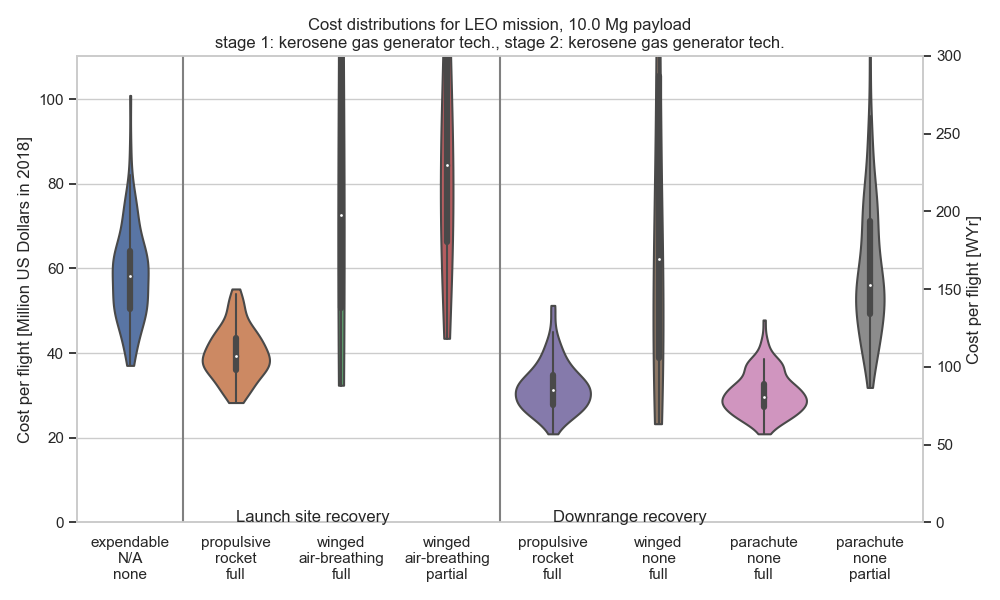
\includegraphics[width=\textwidth]{../../lvreuse/analysis/combined/plots/strategy_cost_LEO_kerosene_pld10000}
    \caption{\label{fig:strategy_cost_LEO_kerosene_pld10000} Cost per flight distributions for various first stage reuse strategies, assuming kerosene technology and carrying a 10 ton payload to LEO. Note that downrange propulsive landing and downrange parachute recovery have the lowest expected costs, and that the cost of winged strategies is highly uncertain.}
\end{figure}

\begin{figure}[hbt!]
    \centering
    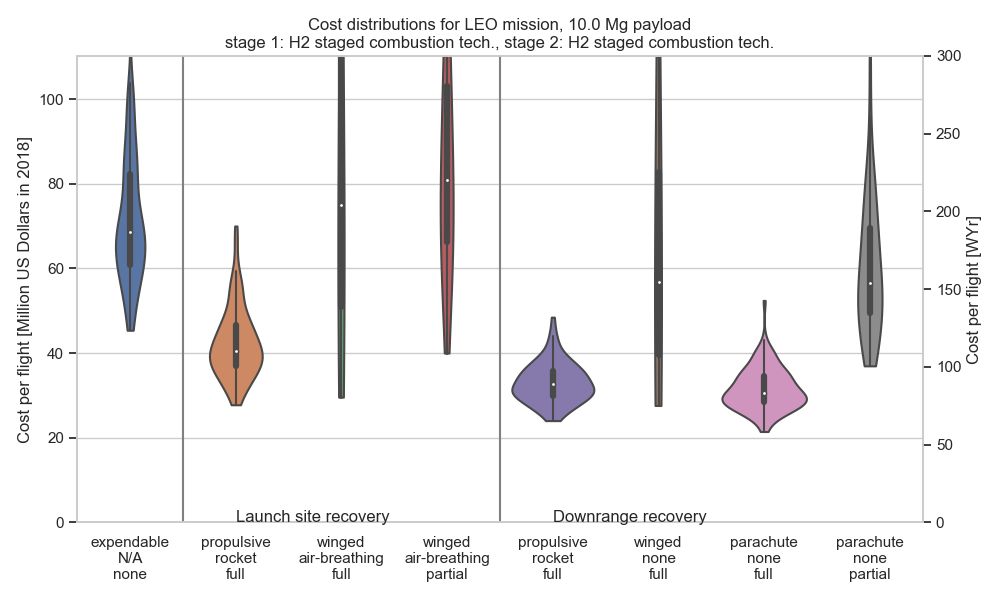
\includegraphics[width=\textwidth]{../../lvreuse/analysis/combined/plots/strategy_cost_LEO_H2_pld10000}
    \caption{\label{fig:strategy_cost_LEO_H2_pld10000} Cost per flight distributions for various first stage reuse strategies, assuming hydrogen technology and carrying a 10 ton payload to LEO. The distributions are similar to those for kerosene, although the expected costs are slightly higher.}
\end{figure}

The downrange propulsive landing and parachute strategies for full first stage recovery show very similar distributions with the lowest cost per flight distributions among all the strategies. However, as mentioned previously, parachute recovery of the full first stage is not very feasible for large vehicles. Therefore downrange propulsive landing is the most effective strategy for achieving the lowest cost per flight. 

We see broad distributions for winged recovery strategies due to a small number of historical reference projects available for fitting the production CER coefficients. This lack of data leads to large uncertainties in the coefficient values, resulting in large uncertainties in the output cost per flight distributions. 

It is also interesting to compare the cost per flight distributions for the two different technology choices (kerosene with gas generator and H2 with staged combustion). Despite the hydrogen technology choice yielding slightly better payload performance, the cost per flight distributions show slightly lower costs for kerosene. This result likely stems from two reasons:

\begin{itemize}
  \item The cost per kilogram of inert mass for producing a vehicle using hydrogen propellant is greater than that for kerosene. 
  \item The inert mass of a vehicle using hydrogen propellant is generally greater than that of kerosene for a given payload mass.
\end{itemize}

Additionally, partial reuse strategies do not seem to yield substantial cost per flight savings relative to full reuse strategies. For these reuse strategies, the extra mass required to make a first stage vehicle partially recoverable does not make up for any cost savings achieved by reusing the high-value components. 

% Maybe include some GTO stuff here if there is room.

\subsection{Effect of number of reuses and launch rate}
In order to look at the breakdown of costs for a launch vehicle with a reusable first stage, we consider a point cost estimate to demonstrate general trends. The following example evaluates a two stage launch vehicle carrying a 10,000 kg payload to LEO using kerosene and liquid oxygen propellants at a launch rate of 15 launches per year. We consider the case of a propulsive downrange landing to recover and reuse the entire first stage. The cost per flight is determined over a range of number of first stage uses. The results of this analysis are shown in Figure \ref{fig:cpf_stackplot_reuses_sweep}.

\begin{figure}[hbt!]
    \centering
    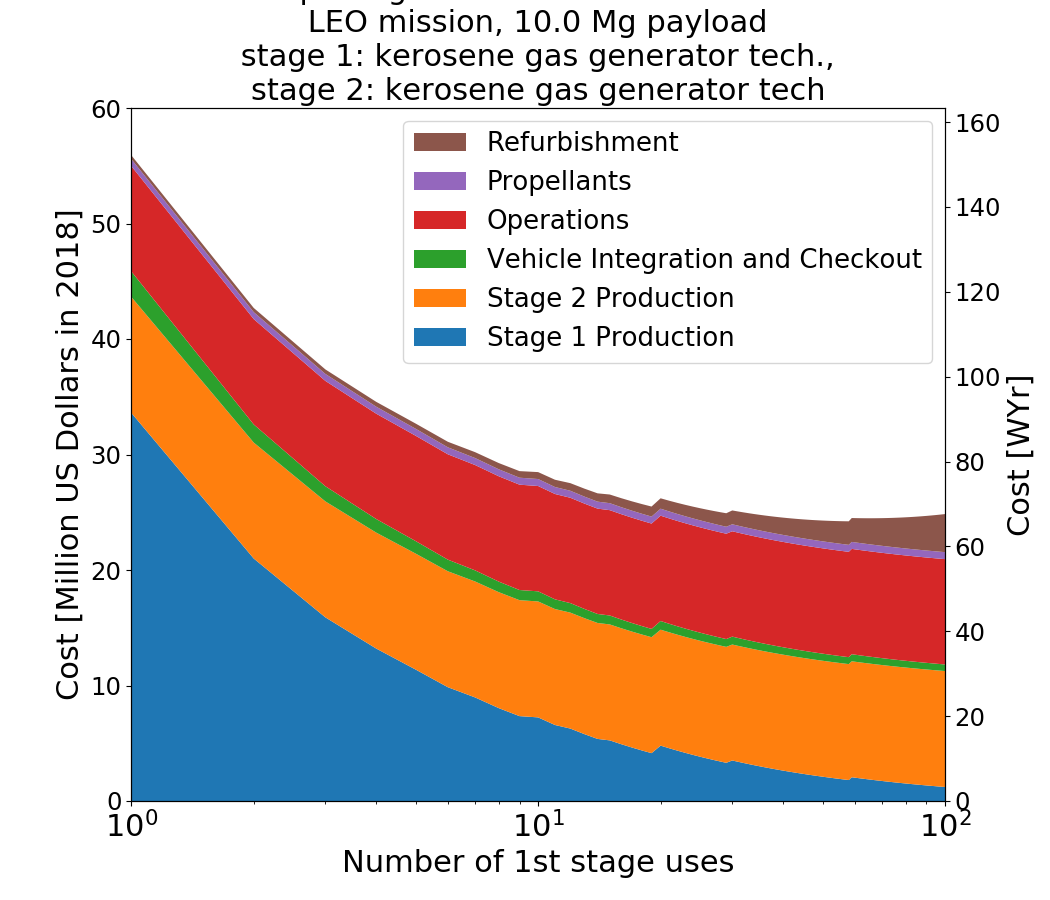
\includegraphics[width=\textwidth]{../../lvreuse/analysis/combined/plots/cpf_stackplot_reuses_sweep}
    \caption{\label{fig:cpf_stackplot_reuses_sweep} A sweep of cost per flight vs number of first stage reuses for an example downrange propulsive landing strategy. Stage 1 production cost per flight declines as the first stage is reused more times. Refurbishment costs make up a small fraction of the cost per flight, but increase with increasing number of reuses.}
\end{figure}

Several things should be noticed from the results in Figure \ref{fig:cpf_stackplot_reuses_sweep}. First, the stage one productions costs per flight decrease dramatically as we increase the number of first stage reuses. This result is very intuitive -- as the cost of first stage production is spread over a larger number of flights, the per flight amortization share of the first stage production cost decreases. This leads to a reduction in the cost per flight. However, this trend of decreasing amortization share of first stage production costs is opposed by the refurbishment cost trends. As the number of first stage uses increases, the refurbishment cost per flight also increases. This is due to the fact that more components on the first stage will need inspected or replaced  as the number of reuses increases. 

These opposing trends lead to an interesting result: the total cost per flight trend achieves a minimum value. Under the assumptions used in Figure \ref{fig:cpf_stackplot_reuses_sweep}, the minimum cost per flight occurs near 60 reuses, but the exact location is highly dependent the model parameters, especially refurbishment costs. Generally though, there will be some number of reuses beyond which further reuse is not cost effective.

The cost per flight is also affected by the annual launch rate. Although most components of the cost per flight do not vary with launch rate, operations costs are very sensitive to it. Launch operations require a dedicated workforce and facilities, which are underutilized at low launch rates. Therefore we see a higher operations cost per flight at low launch rates. The cost per flight trends with varied launch rates are given in Figure \ref{fig:cpf_reuses_sweep_vary_launch_rate}. 

\begin{figure}[hbt!]
    \centering
    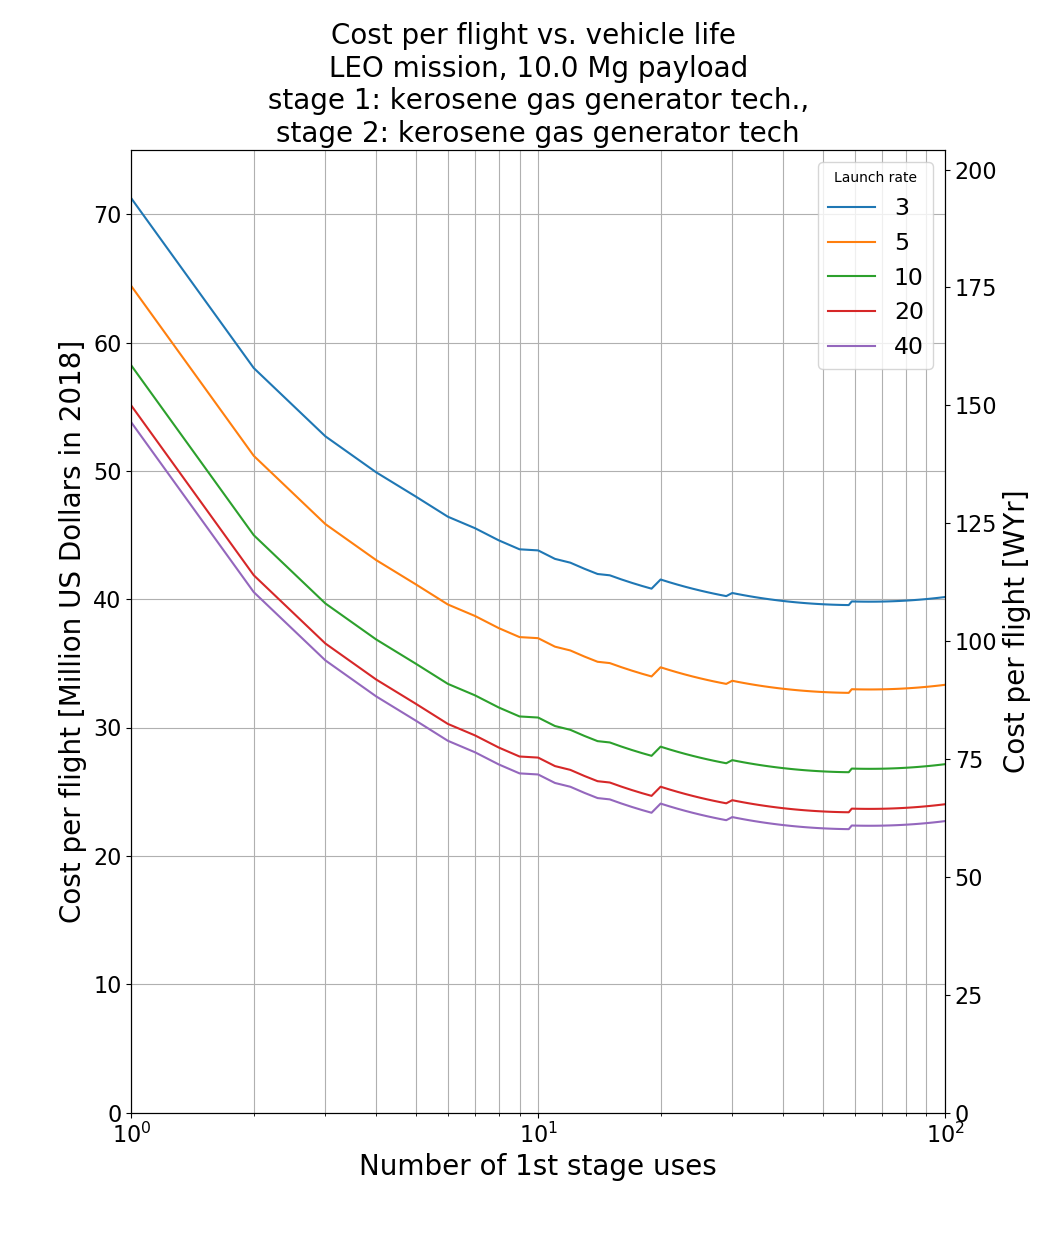
\includegraphics[width=\textwidth]{../../lvreuse/analysis/combined/plots/cpf_reuses_sweep_vary_launch_rate}
    \caption{\label{fig:cpf_reuses_sweep_vary_launch_rate} The cost per flight vs. number of reuses sweep repeated at several launch rates. Increasing launch rate decreases cost per flight (primarily through lower operational costs) but the benefits diminish past about 20 launches/year.}
\end{figure}

As expected, Figure \ref{fig:cpf_reuses_sweep_vary_launch_rate} shows that the cost per flight is higher at lower launch rates, regardless of the number of first stage reuses. For low launch rates, we see a substantial decrease in the cost per flight for only a modest increase in launch rate. However, for high launch rates, further increases in launch rate do not have a large effect on the cost per flight. For instance, we see a large difference in cost per flight by increasing the launch rate from 3 to 5 launches per year. However, increasing the launch rate from 20 to 40 launches per year yields only minimal cost per flight reductions. 

We next consider some of these cost per flight trends for various first stage reuse strategies. Figure \ref{fig:num_reuse_sweep_LEO_kerosene} shows the costs per flight for selected strategies over a range of number of first stage uses. We consider two cases in this analysis: 

\begin{itemize}
  \item First stage reuse has no effect on the vehicle launch rate. The first stage production rate is not a rate-limiting step of the launch rate. In this case, a production and launch rate of 15 vehicles per year. 
  \item First stage reuse allows the launch rate to increase beyond the first stage production rate. For illustration, we assume that the first stage production rate is 15 stages per year, and that in this case the launch rate is $min(15 * n_{reuse}, 50)$
\end{itemize}

For all strategies, we see a decrease in the cost per flight as the number of first stage uses increases. This result is not surprising -- increasing the launch rate decreases the operations cost per flight. It is interesting though to compare the strategy cost per flight trends with the cost of an expendable vehicle. For the strategies considered in Figure \ref{fig:num_reuse_sweep_LEO_kerosene}, all but the partial parachute recovery strategy show costs per flight below the 10th percentile of expendable cost per flight estimates above a certain number of reuses. With partial parachute recovery, the high-value hardware reuse savings do not compensate for the additional costs of producing and operating a reusable vehicle. However, the other strategies show potential for significant cost per flight savings with a high enough number of first stage reuses. 

\begin{figure}[hbt!]
    \centering
    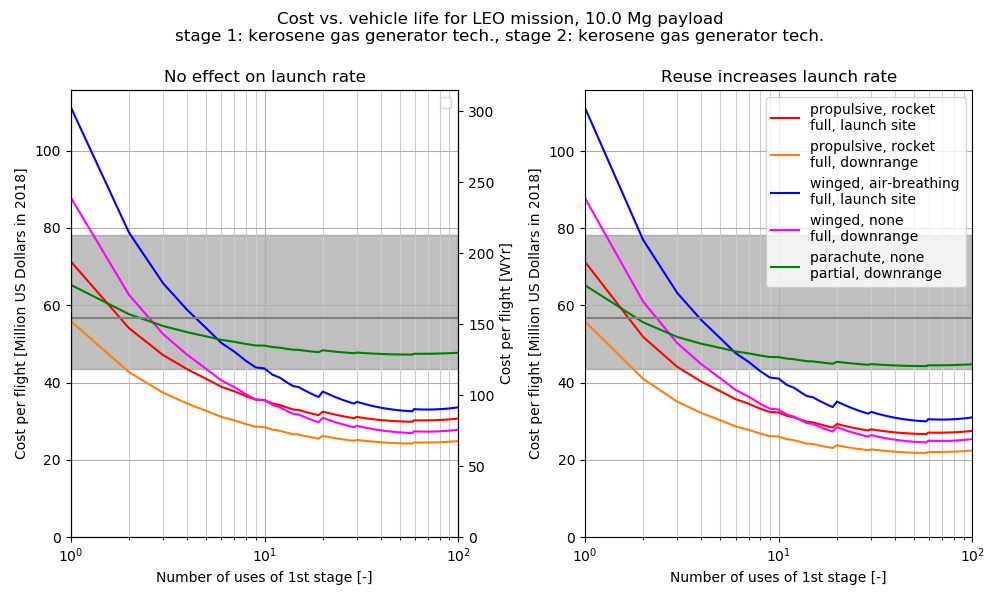
\includegraphics[width=\textwidth]{../../lvreuse/analysis/combined/plots/num_reuse_sweep_LEO_kerosene}
    \caption{\label{fig:num_reuse_sweep_LEO_kerosene} The cost per flight vs. number of reuses sweep, repeated for various reuse strategies. For comparison, the grey bar shows the expendable cost distribution's \nth{10} to \nth{90} percentiles.}
\end{figure}

\subsection{Effect of launch vehicle size}

The potential for cost per flight savings of first stage reusability is highly dependent on the payload or vehicle size. In the previous discussion, we considered the case of a 10 Mg payload to LEO. The cost per flight breakdown for this case shown in Figure \ref{fig:cpf_stackplot_reuses_sweep} shows that first stage production costs make up the majority of costs in the expendable case, and that first stage reuse can lead to significant cost per flight savings. However, the cost per flight breakdown looks very different for a smaller payload. 

Let's consider the case of a small 100 kg payload to LEO. As can be seen in Figure \ref{fig:cpf_stackplot_reuses_sweep_small_sat}, first stage production costs no longer make up the majority of the cost per flight since costs for small launch vehicles are not dominated by hardware costs. Instead, the operations costs make up the majority of the cost per flight. The operations costs per flight are largely independent of vehicle and payload mass, and therefore do not decrease substantially as the payload and vehicle mass decrease. For these reasons, first stage reusability for small launch vehicles is impractical. Amortizing the first stage production costs for a small launch vehicle over a number of flights does not lead to large cost per flight savings since the production costs were already a small fraction of the cost per flight.

\begin{figure}[hbt!]
    \centering
    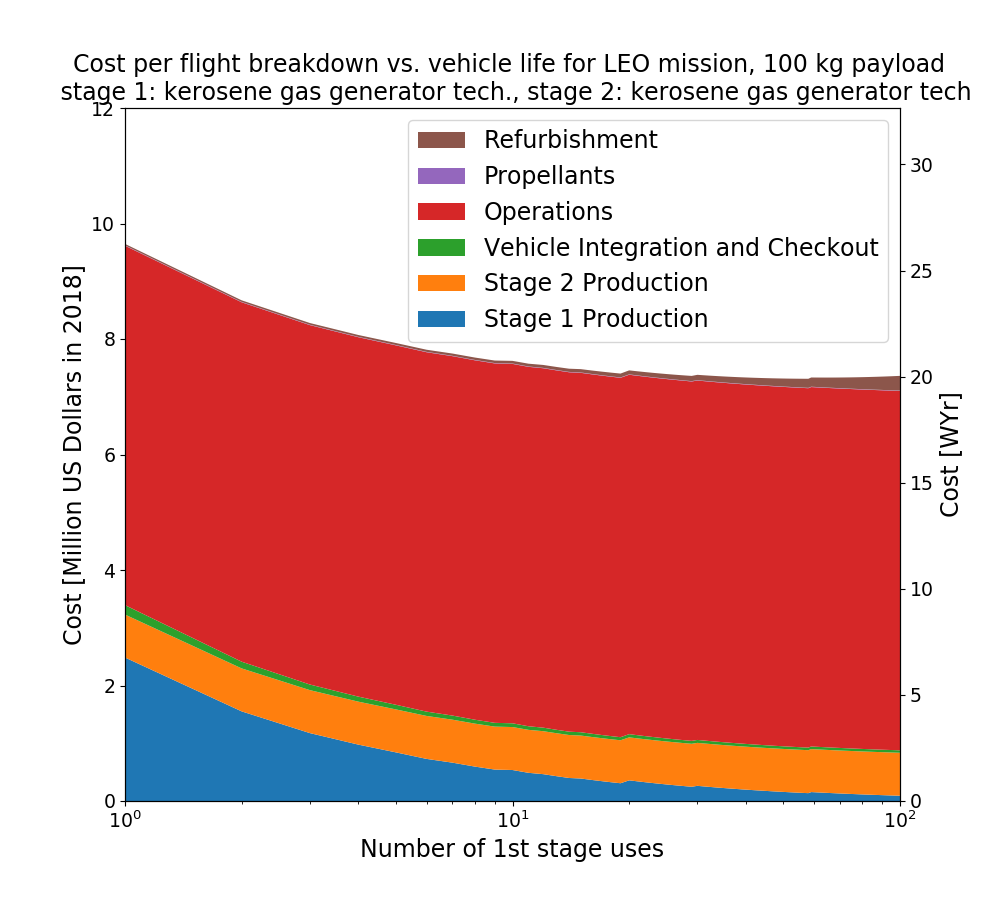
\includegraphics[width=\textwidth]{../../lvreuse/analysis/combined/plots/cpf_stackplot_reuses_sweep_small_sat}
    \caption{\label{fig:cpf_stackplot_reuses_sweep_small_sat} The cost per flight of a small launcher (100 kg payload) is expected to be dominated by operations costs, and does not decline meaningfully with first stage reuse.}
\end{figure}

We next consider the cost per kilogram payload per flight over a range of payload masses, as given in Figure \ref{fig:m_payload_sweep_LEO_kerosene}. This plot reveals a trend of decreasing cost per kilogram payload per flight as payload mass -- and therefore vehicle size -- increases. More interesting though is that the spread between the estimates of cost per kilogram payload per flight increases with increasing payload mass and launch vehicle size. 

As previously discussed, the cost per flight for small vehicles is not dominated by vehicle hardware costs. Even though there are differences in payload mass fractions (TODO ref performance section/violin plots) between strategies, these differences are relatively inconsequential in estimating cost per flight for small vehicles since hardware mass was not a strong cost driver anyway. However, for increasing payload vehicle size, hardware costs make up a larger fraction of the cost per flight. Therefore, as the vehicle size increases, we see the cost per flight per mass payload estimates for the different reuse strategies diverge as differences in payload performance become more important in determining costs. 

\begin{figure}[hbt!]
    \centering
    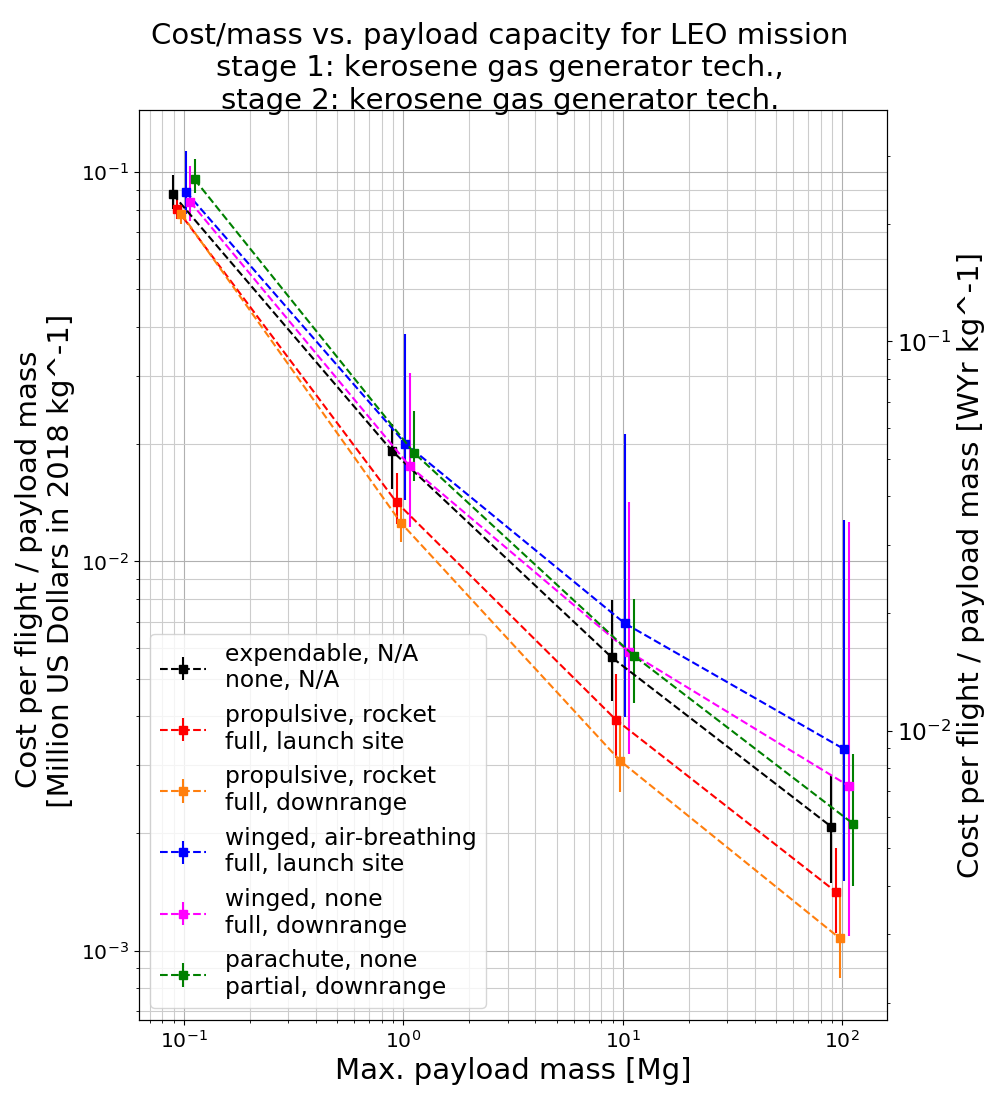
\includegraphics[width=\textwidth]{../../lvreuse/analysis/combined/plots/m_payload_sweep_LEO_kerosene}
    \caption{\label{fig:m_payload_sweep_LEO_kerosene} As payload mass increases, the cost/mass spread between reuse strategies widens. The error bars on each point show the \nth{10} to \nth{90} percentiles of the cost/mass estimate. The points are "jittered" on the x-axis for visual clarity.}
\end{figure}

\subsection{Paying off development costs}

In our models and discussion so far, we have yet to consider the development costs of the reuse strategies. The development costs of reusable launch vehicles can generally be expected to be greater than a similar expendable vehicle. However, the cost per flight savings for reusable vehicles can also be substantial, as shown in Figure \ref{fig:num_reuse_sweep_LEO_kerosene}. These opposing trends lead to an important question: do the cost per flight savings of reusable launch vehicles pay off their increased development costs? 

We address this question by comparing the present value of the savings brought by reusability to the reusable vehicle development costs. In Figure \ref{fig:reuse_npv}, we evaluate the present value of the savings for different launch rates over a range of cost per flight ratios, or the ratio between the cost per flight of a vehicle with first stage reuse and the cost per flight of an expendable vehicle. Credible ranges of development costs and cost per flight ratios are highlighted.

The vehicle launch rate determines how quickly the cost per flight savings for reusability are accrued. With higher launch rates, savings are realized sooner, the present value of the savings is larger, and the investment in reuse development can be paid off faster. This is why we see steeper trends for the present value of savings with higher launch rates. 

In order for a strategy to be economically viable, the present value of the savings must exceed the vehicle's development costs. This seems unlikely for low launch rates -- savings will be realized slowly such that development costs will be greater than the present value of the savings. However, for high launch rates greater than 20 launches per year, first stage reusability appears economically viable. Increased launch rates both reduce the cost per flight and enable the development investment to be paid off sooner. This leads to a higher present value of reuse cost per flight savings, such that the development costs could feasibly be paid off.

\begin{figure}[hbt!]
    \centering
    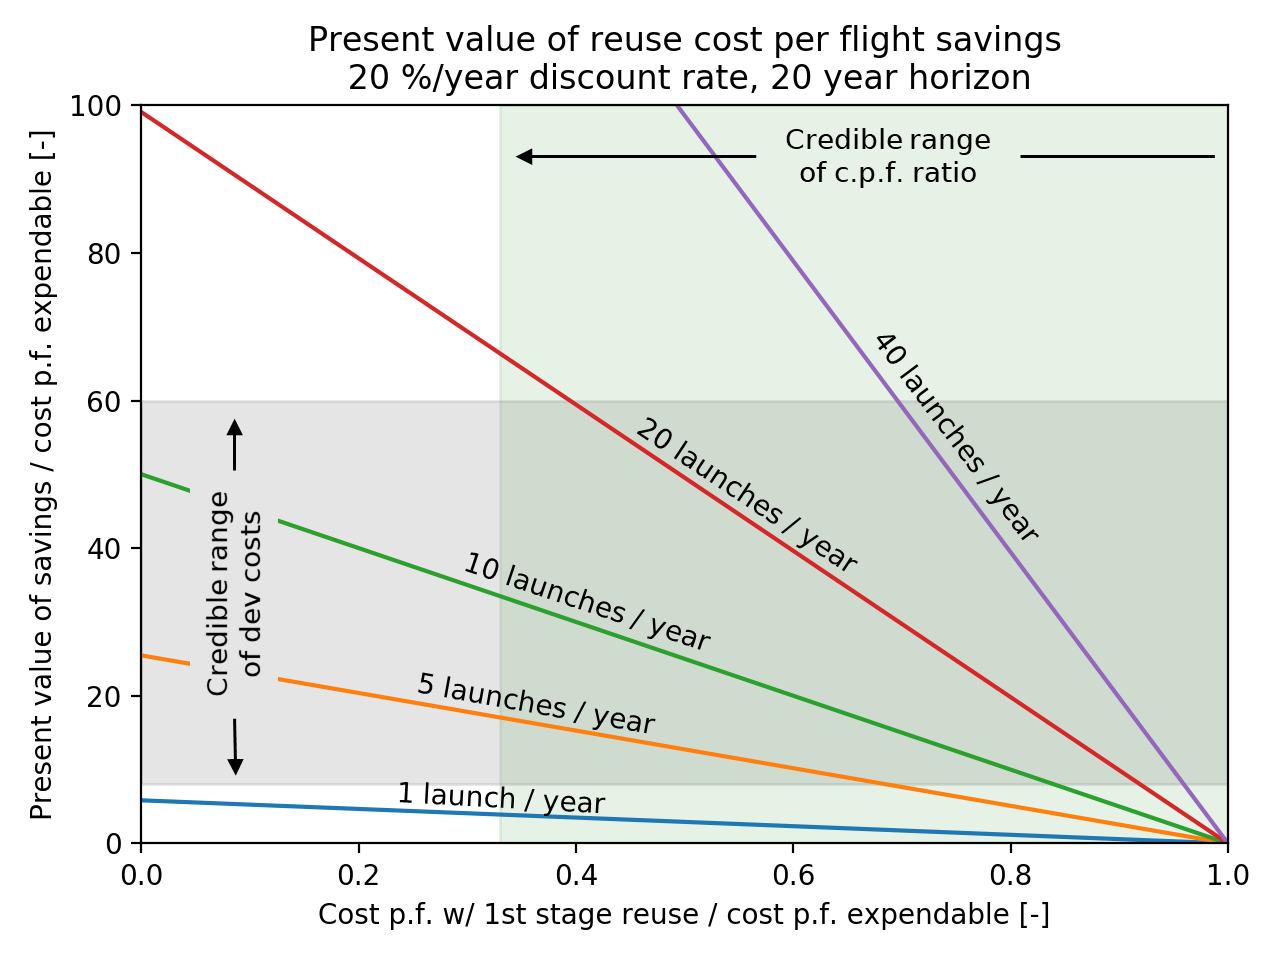
\includegraphics[width=\textwidth]{reuse_npv}
    \caption{\label{fig:reuse_npv} The present value of the cost savings from reuse is higher at higher launch rates.}
\end{figure}

\bibliography{first_stage_recovery}

\end{document}